\section{Risultati}\label{sec:results}

\begin{figure}[H]
    \centering
    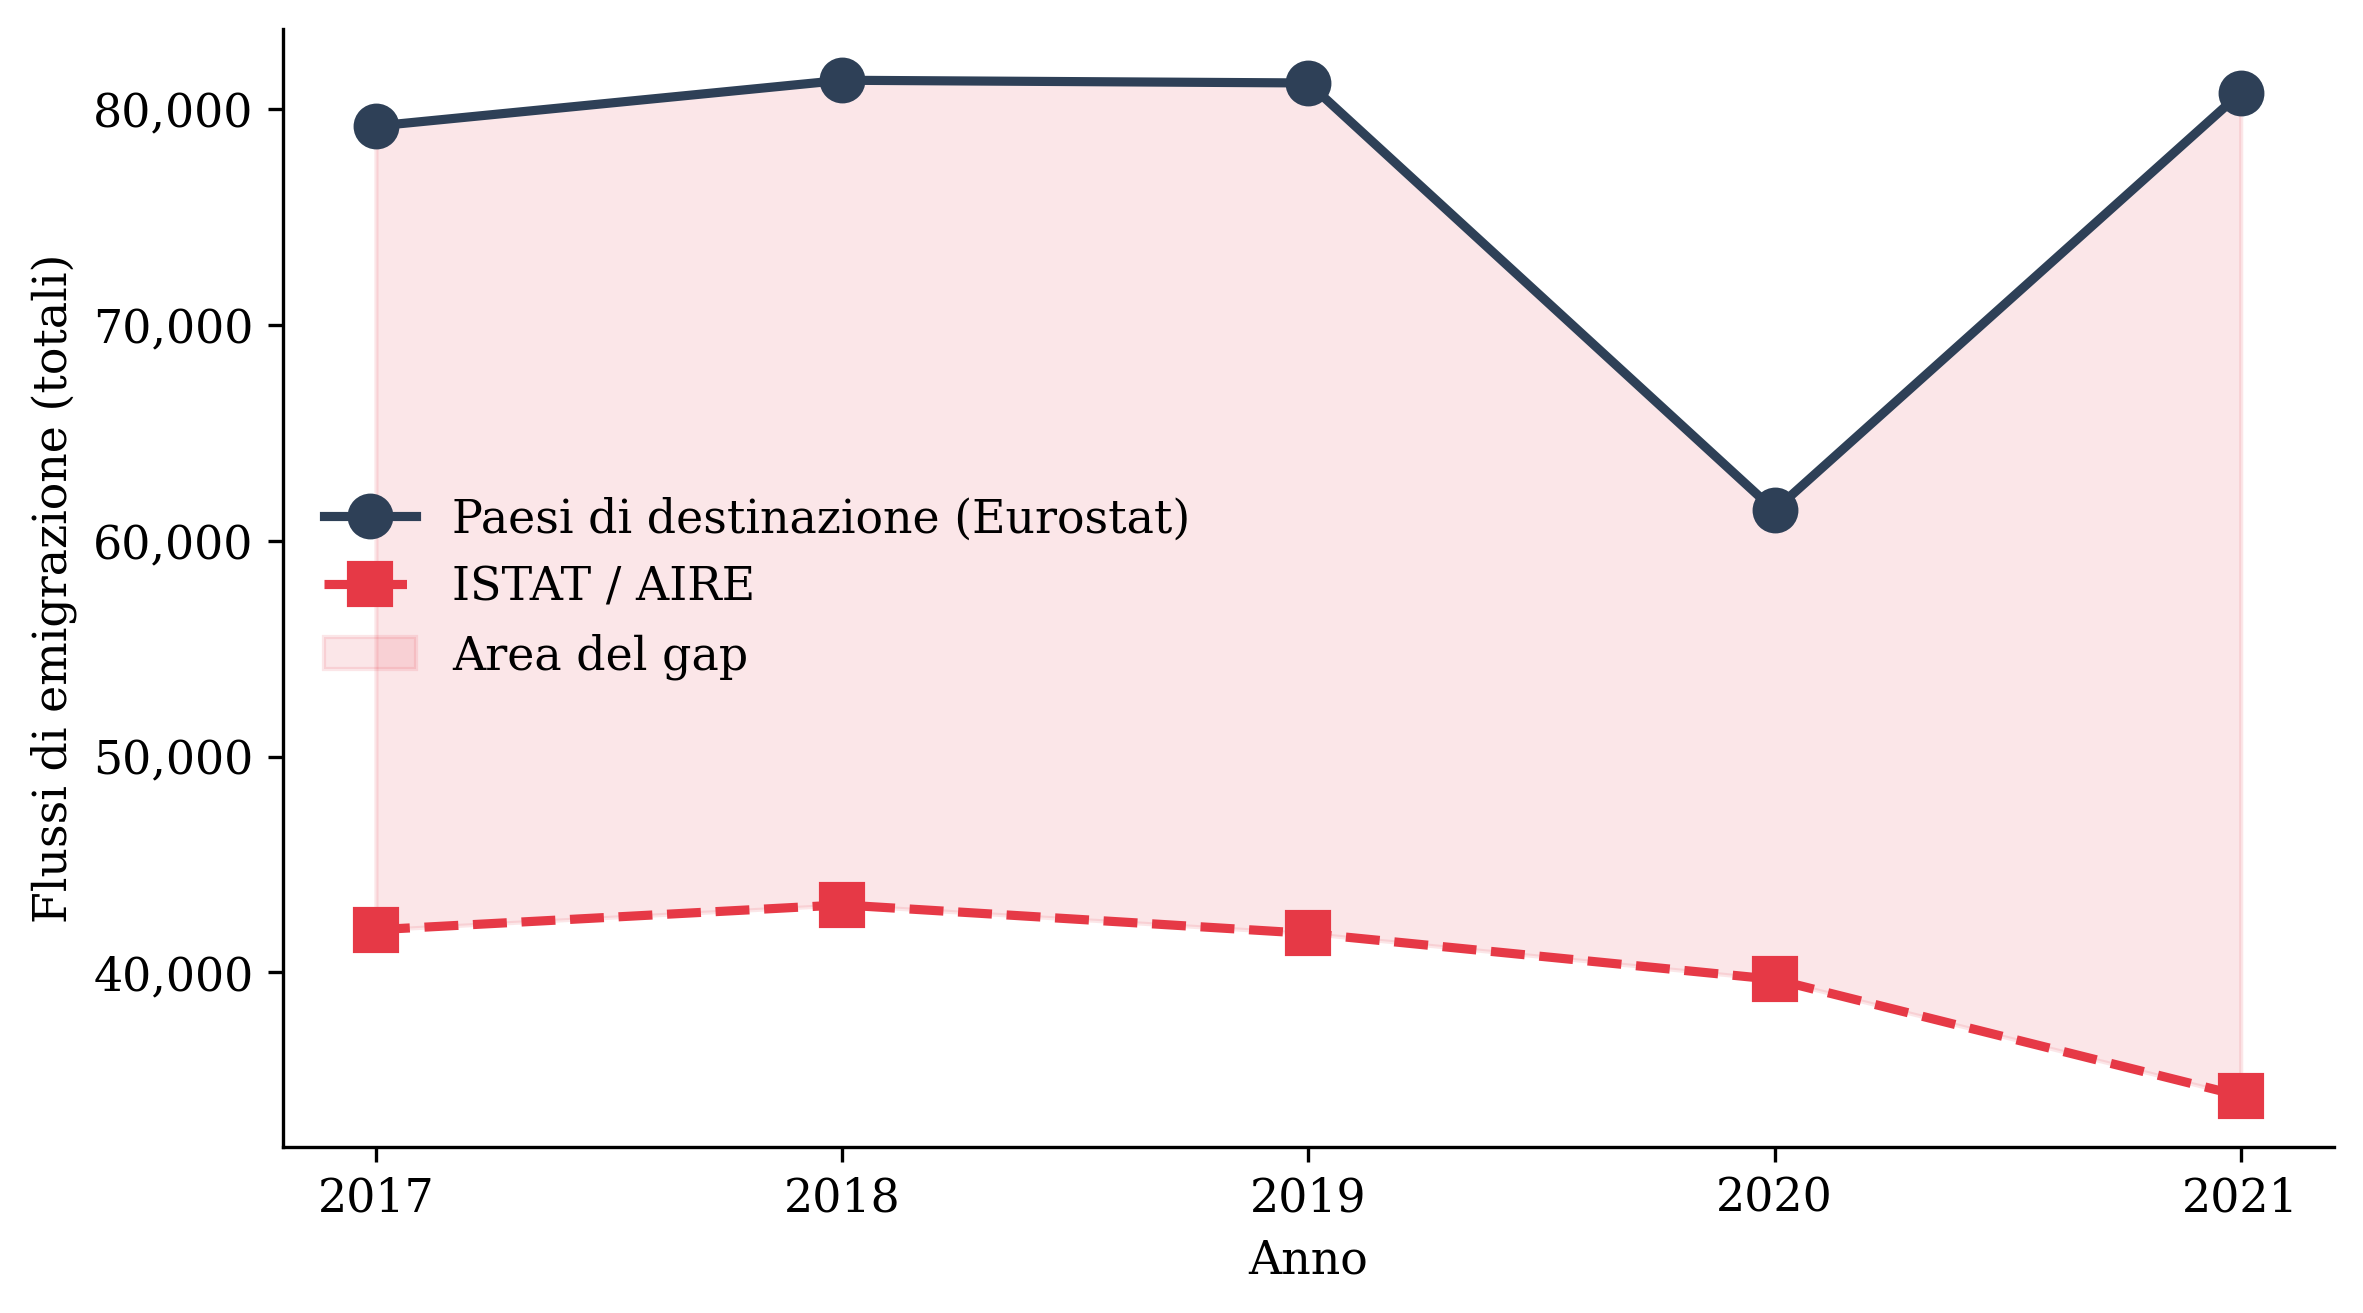
\includegraphics[width=\linewidth]{scripts/figures/fig1_trend}
    \caption{Flussi di emigrazione aggregati per anno: record ISTAT/AIRE rispetto alle registrazioni dei paesi di destinazione.
L'area ombreggiata rappresenta la sottostima sistematica.}
    \label{fig:trend}
\end{figure}

\begin{figure}[H]
    \centering
    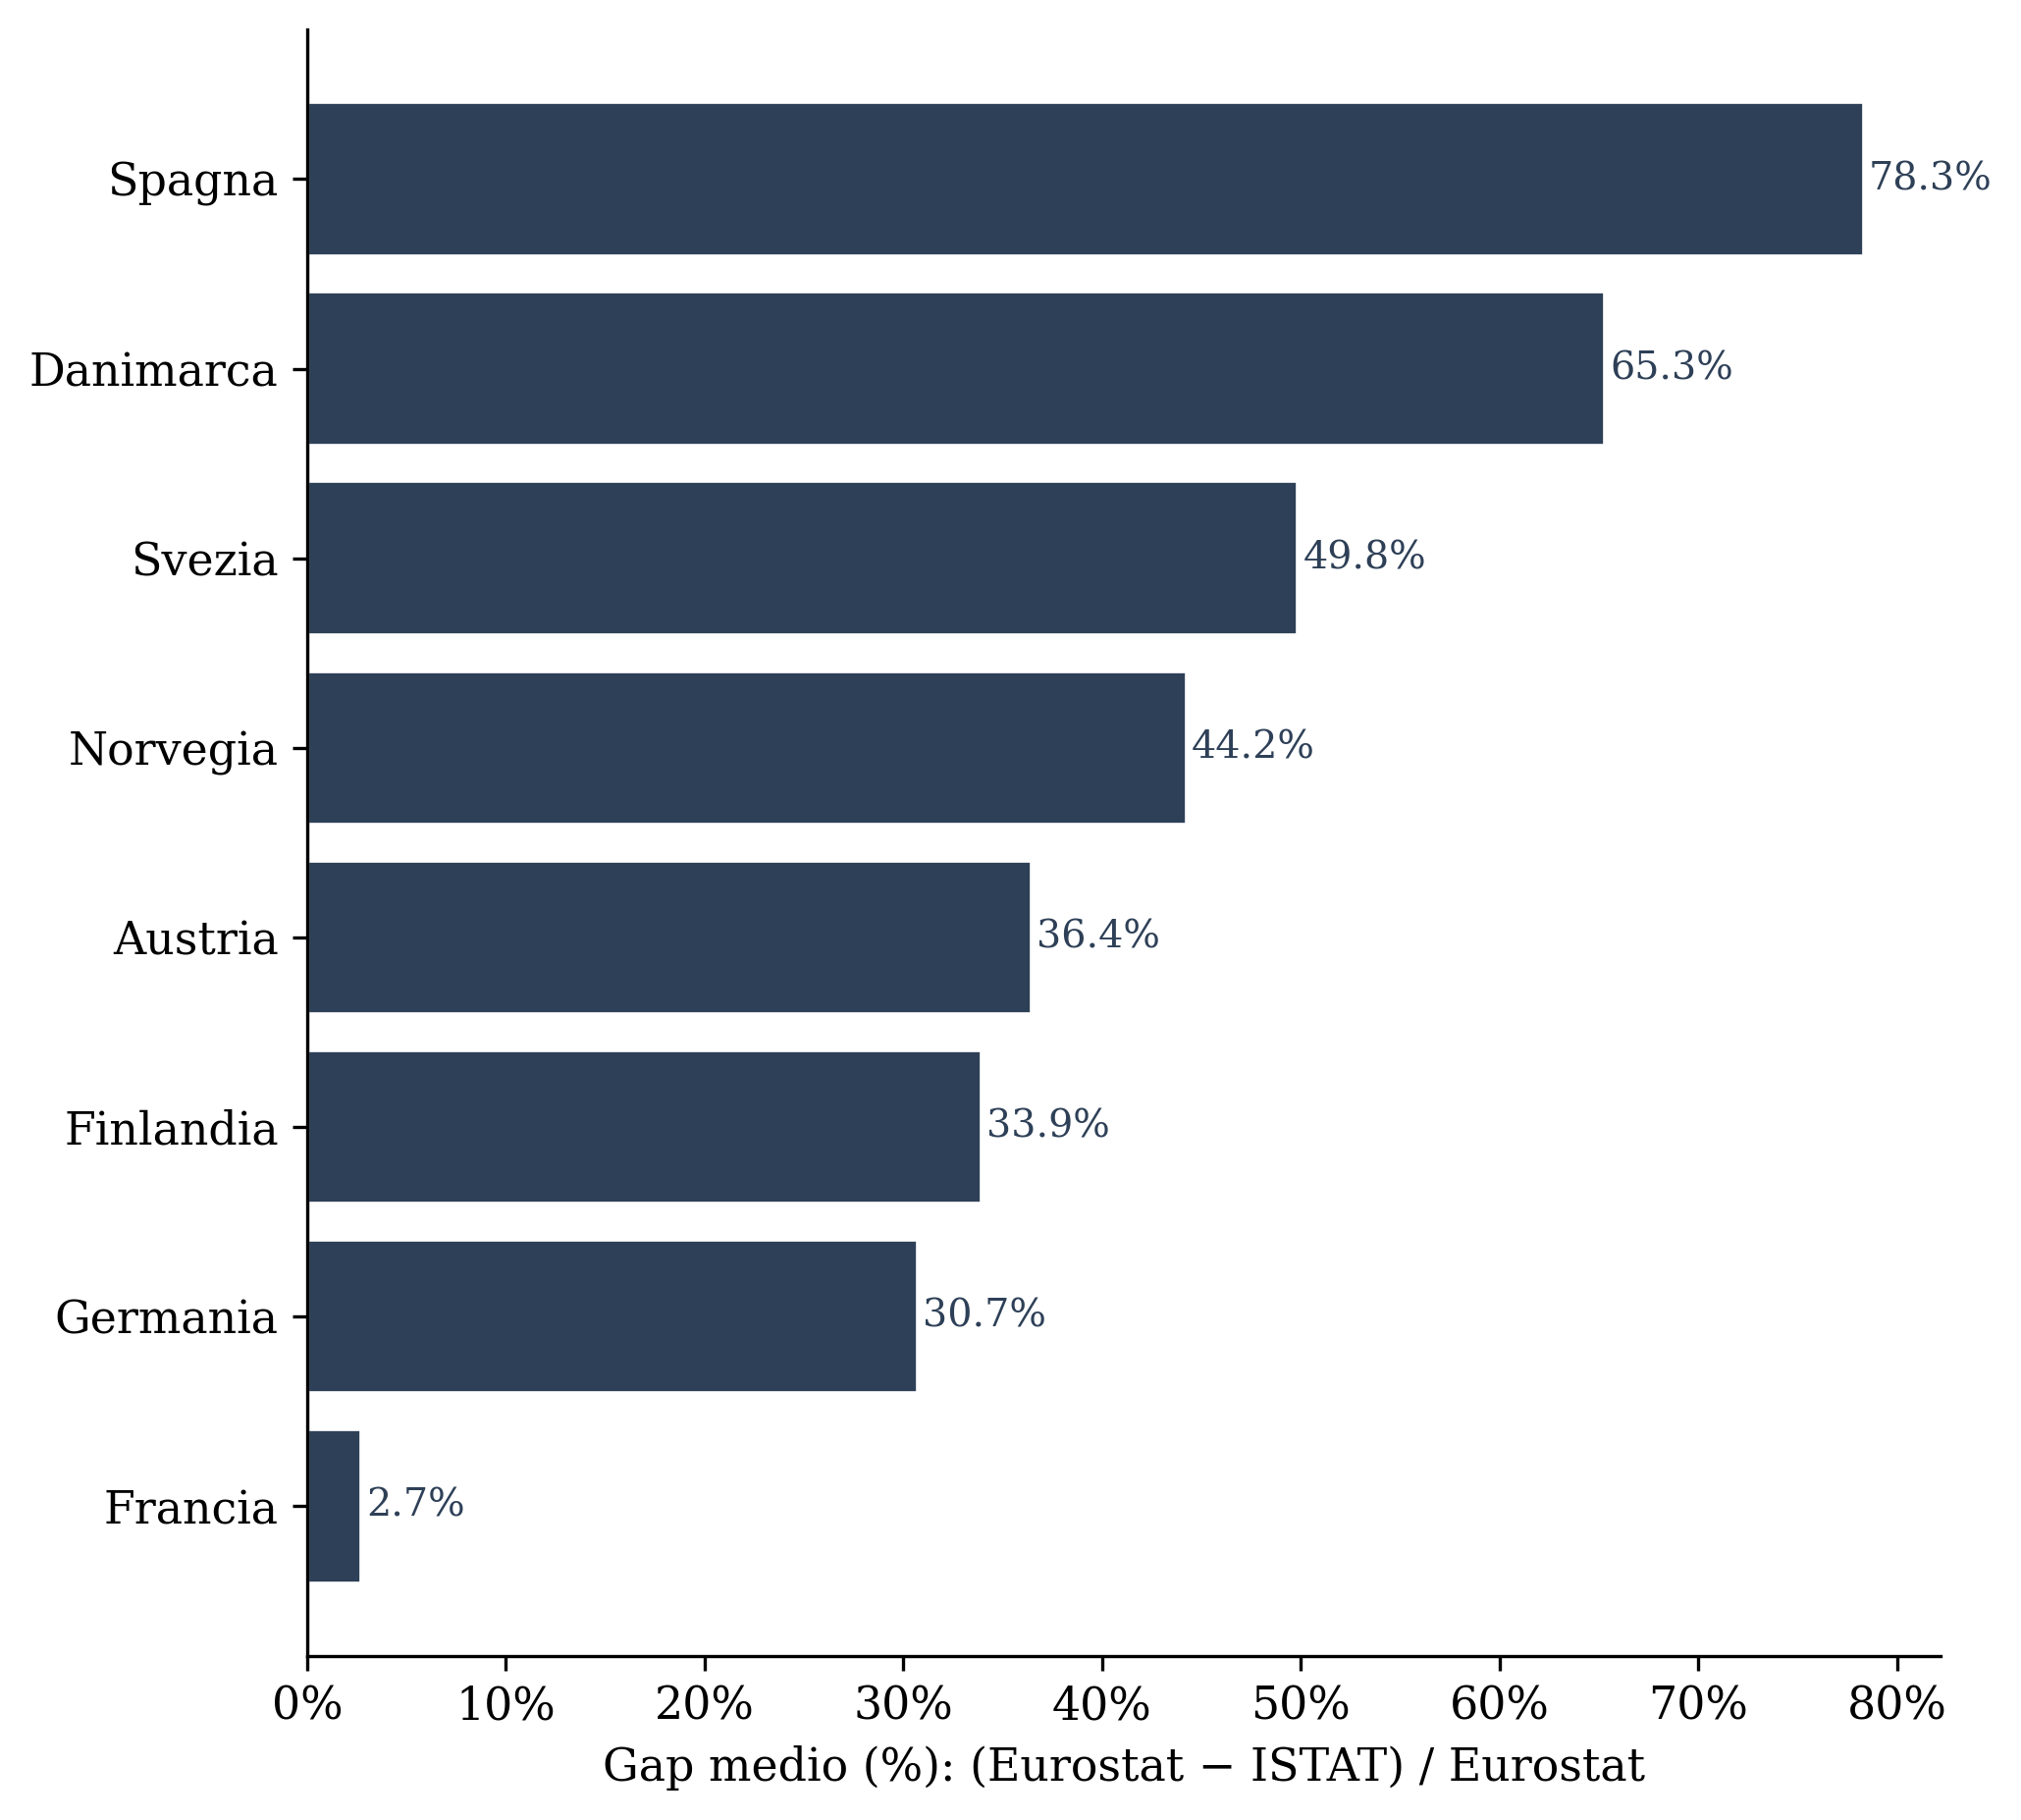
\includegraphics[width=0.85\linewidth]{scripts/figures/fig2_gap_by_country}
    \caption{Tasso medio di sottostima per paese di destinazione.}
    \label{fig:gap_country}
\end{figure}

\begin{figure}[H]
    \centering
    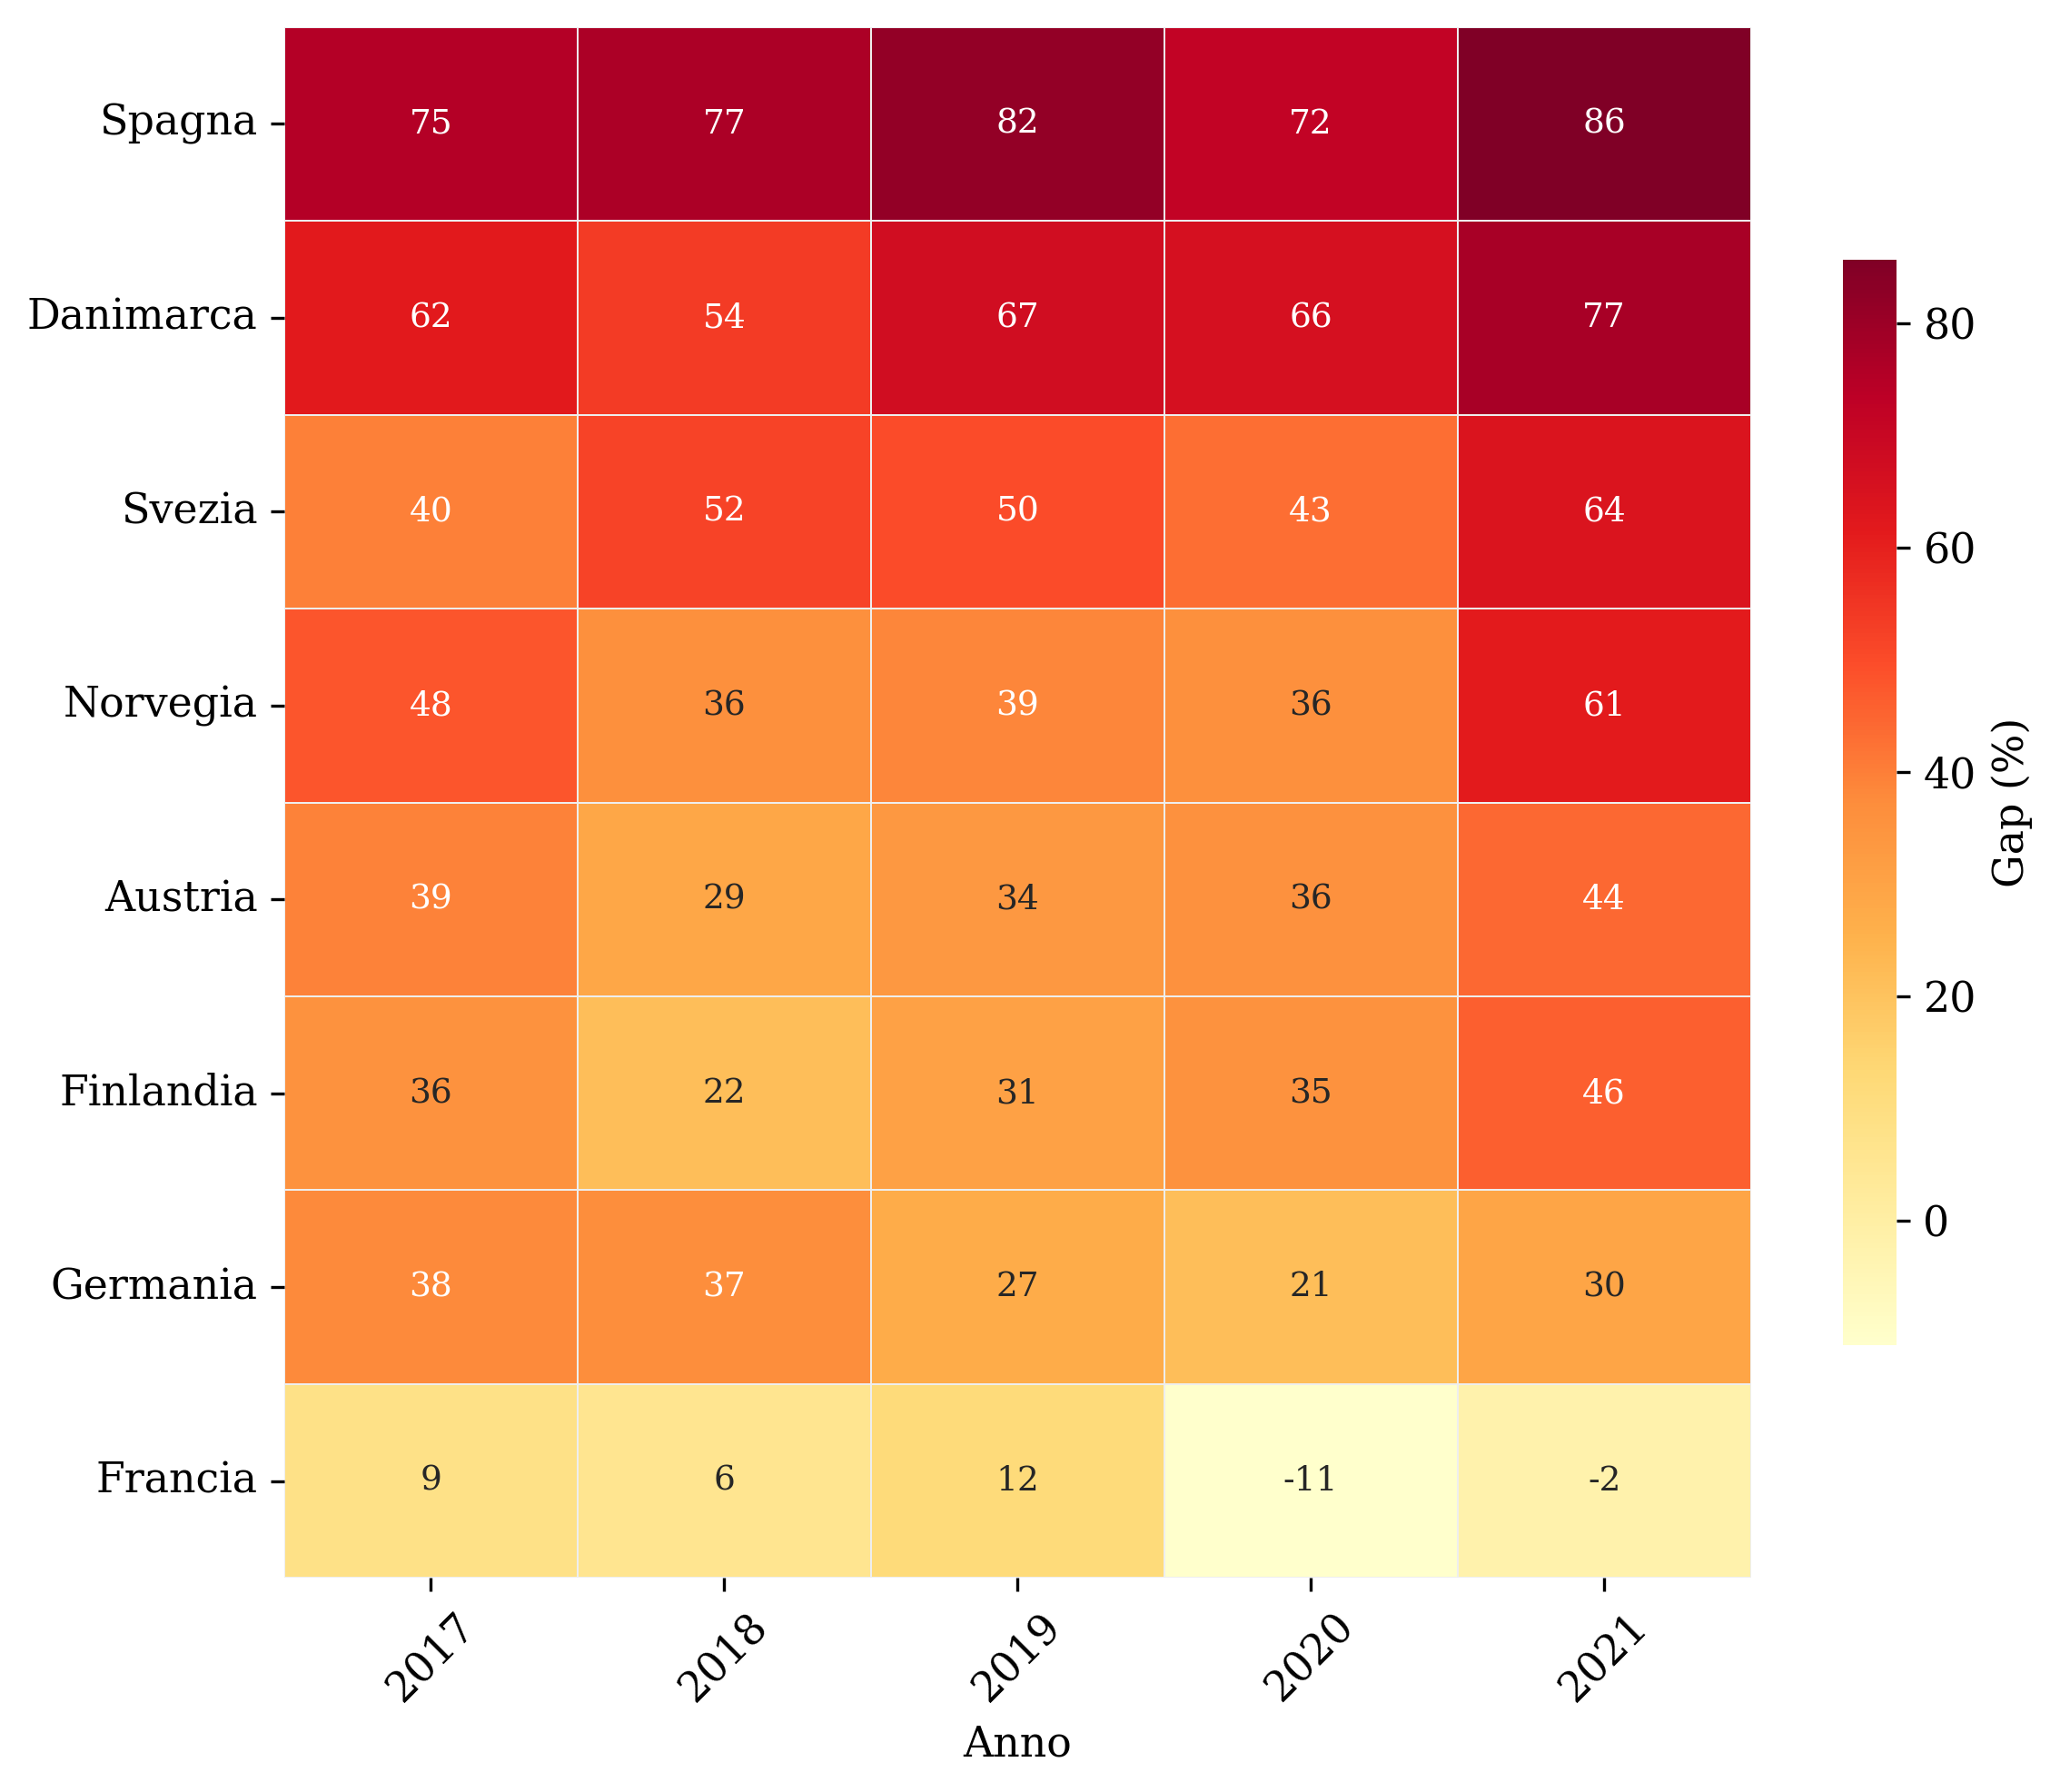
\includegraphics[width=\linewidth]{scripts/figures/fig3_heatmap}
    \caption{Tasso di sottostima (\%) per paese e anno.
Le celle più scure indicano una quota maggiore di emigranti non registrati.}
    \label{fig:heatmap}
\end{figure}

\begin{figure}[H]
    \centering
    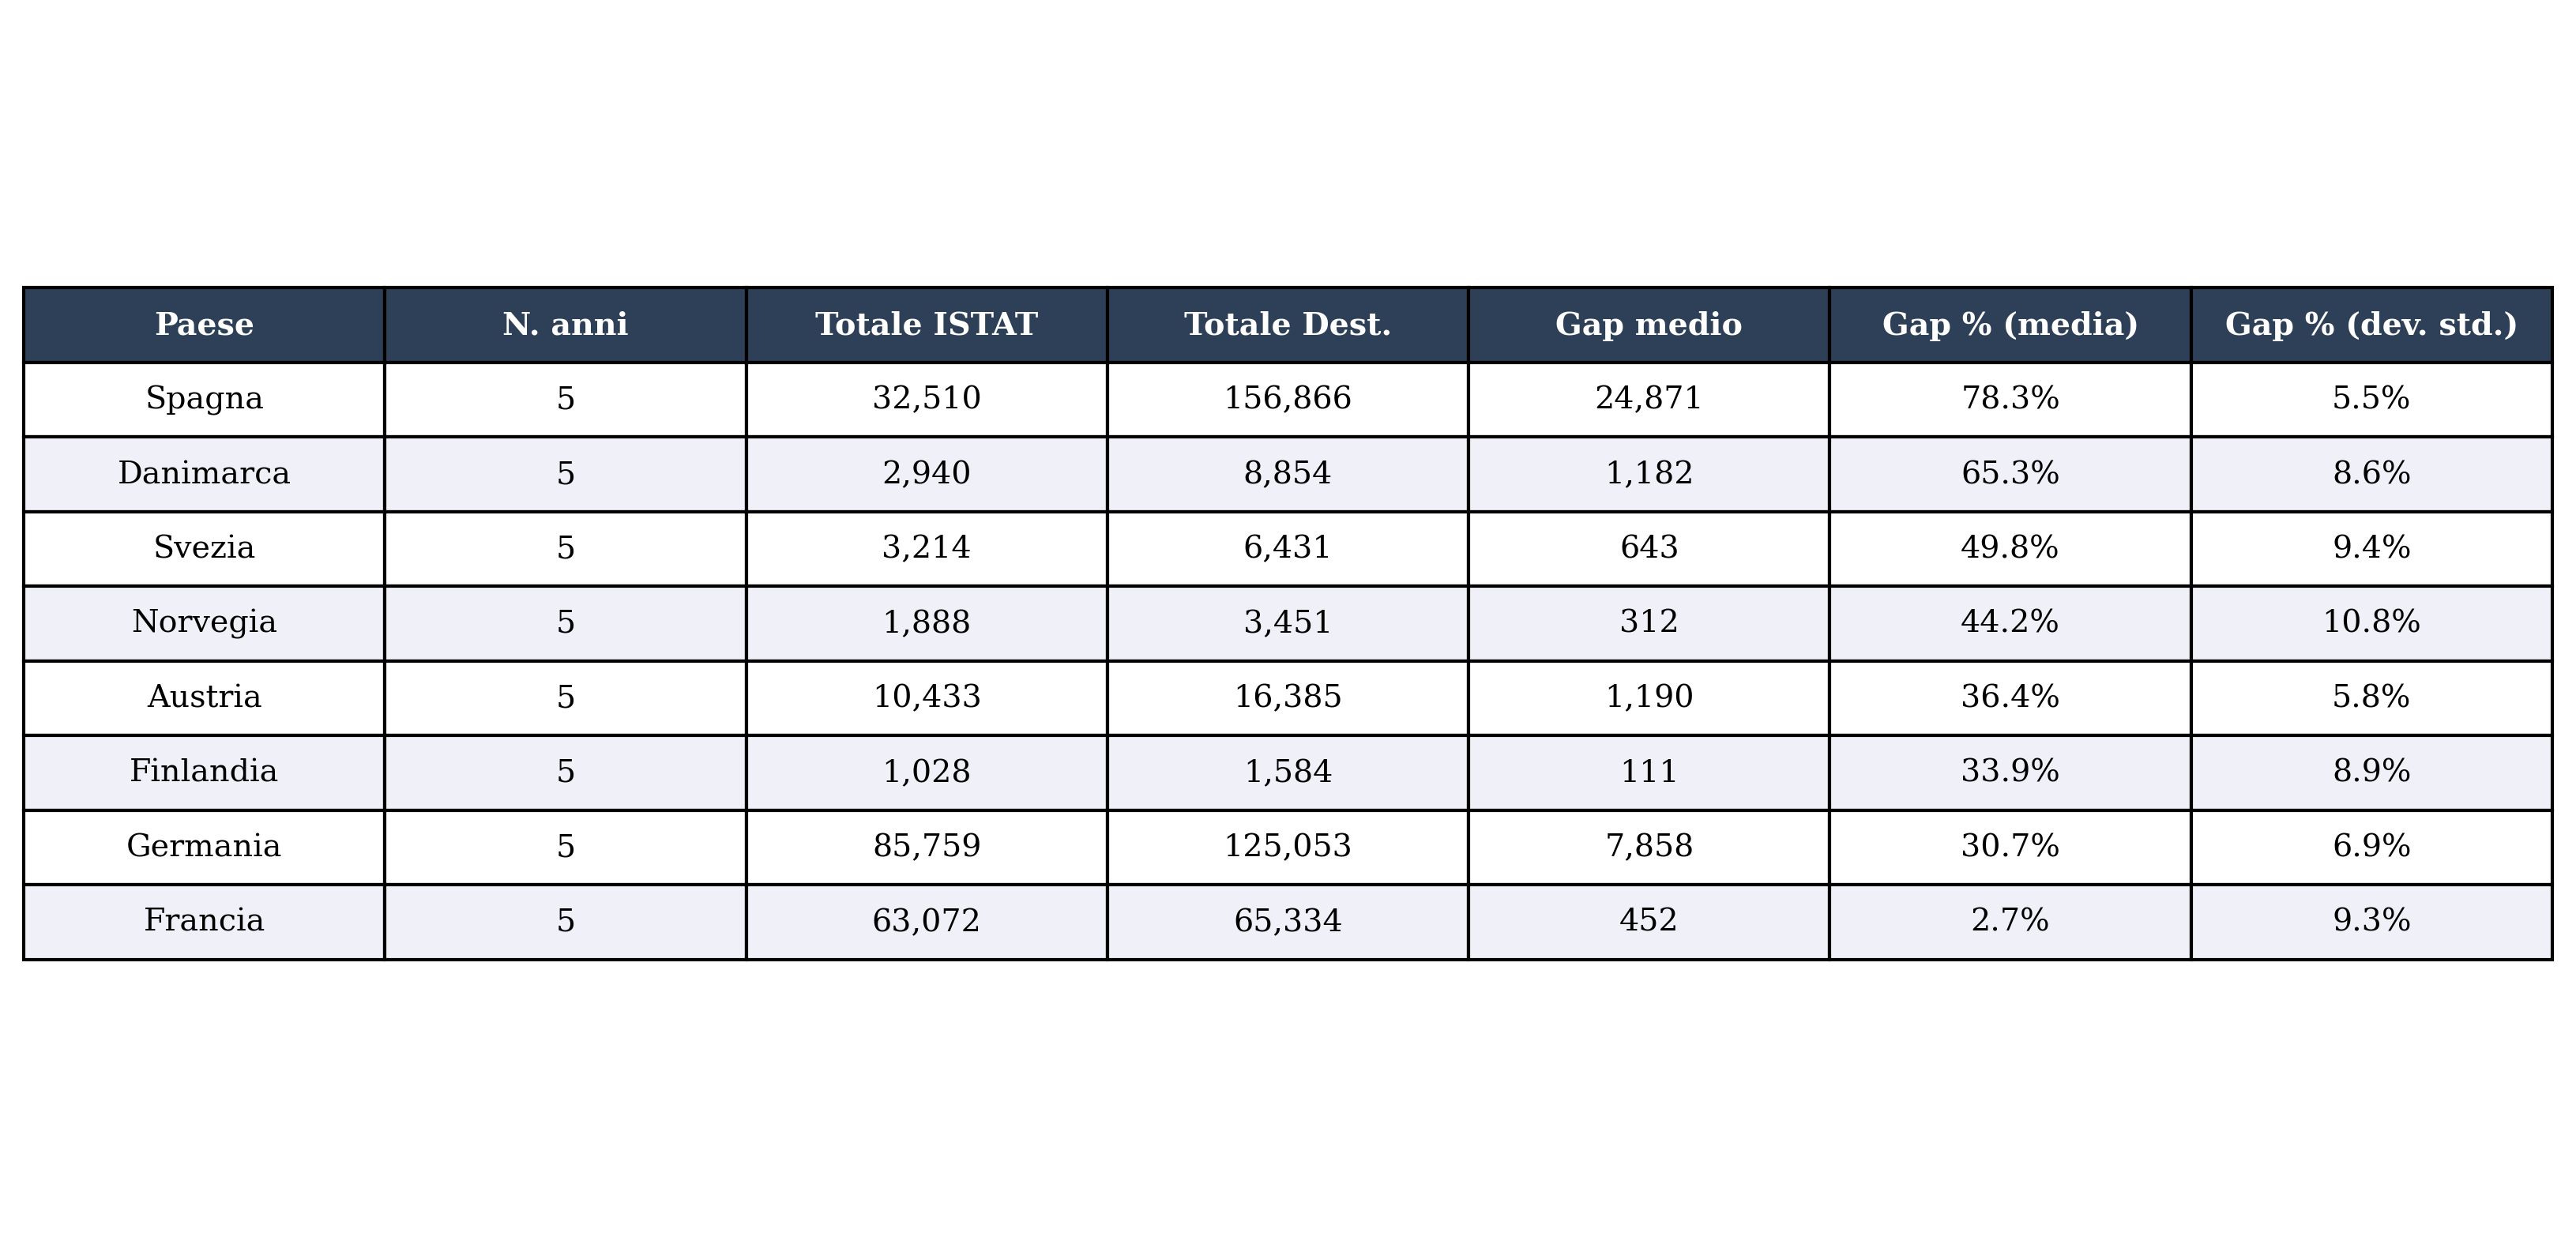
\includegraphics[width=\linewidth]{scripts/figures/fig4_table}
    \caption{Statistiche riassuntive per paese di destinazione: flussi totali, gap medio assoluto e tasso medio di sottostima con deviazione standard.}
    \label{fig:summary_table}
\end{figure}

\begin{figure}[H]
    \centering
    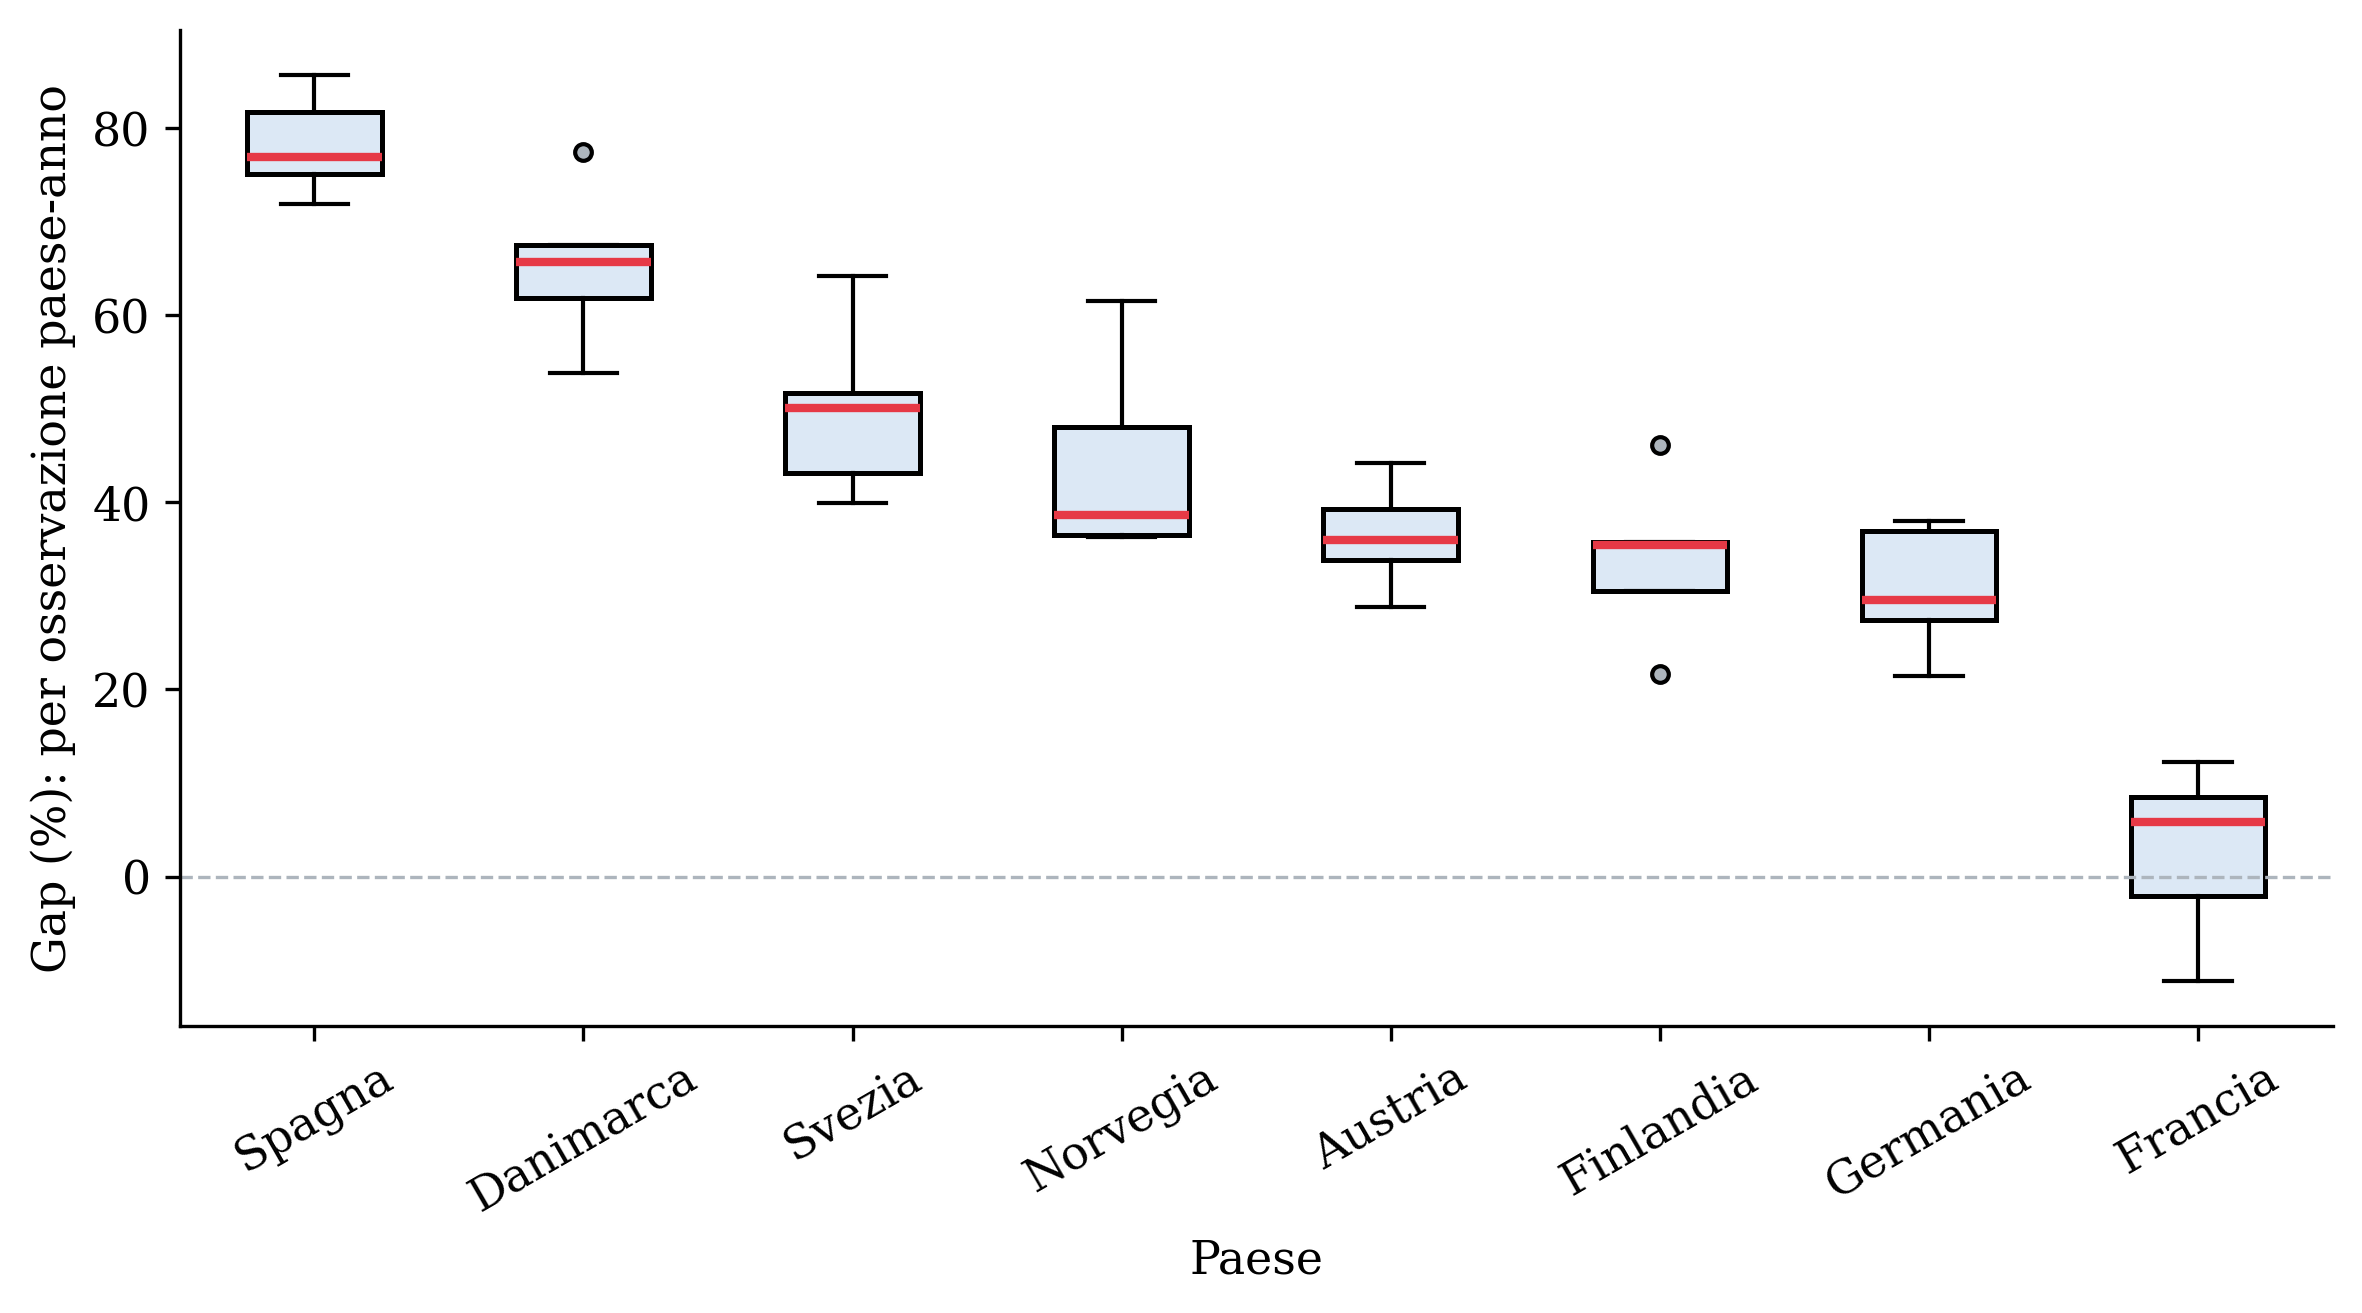
\includegraphics[width=\linewidth]{scripts/figures/fig5_boxplot}
    \caption{Distribuzione del tasso di sottostima per paese.}
    \label{fig:boxplot}
\end{figure}

\subsection{Bias di Volume: Risultati del Test di Wilcoxon}
I risultati del test di Wilcoxon forniscono prove schiaccianti di una sottostima strutturale nei dati amministrativi italiani.
A livello globale (valutando tutte le 40 osservazioni paese-anno), il test restituisce un risultato altamente significativo ($W = 34.0$, $p \approx 4.3 \times 10^{-7}$).
Rifiutiamo l'ipotesi nulla di un gap mediano pari a zero.
In quasi ogni singola osservazione, il dato Eurostat supera significativamente quello ISTAT, generando un diffuso gap positivo (Figura~\ref{fig:trend} e Figura~\ref{fig:gap_country}).
Il test aggregato per paese ($N=8$, sommando i flussi sui 5 anni) conferma ulteriormente questa dinamica, restituendo una statistica di test $W = 0.0$ ($p < 0.01$).
Ciò indica che nell'intero periodo 2017–2021, ogni singolo paese di destinazione analizzato ha ricevuto più cittadini italiani di quanti l'ISTAT ne abbia registrati come emigrati.
In particolare, la statistica del test globale ($W = 34.0$) si discosta dallo zero assoluto esclusivamente a causa di un'anomalia nei dati della Francia durante il biennio 2020–2021. In quei due anni specifici, l'ISTAT ha effettivamente riportato flussi di emigrazione \emph{superiori} a quelli delle autorità francesi.
Questa è l'unica istanza nel nostro dataset in cui il gap è negativo, evidenziando un'interazione unica tra la pandemia e i meccanismi di reporting amministrativo locale (approfondita nella Sezione~\ref{sec:discussion}).
\subsection{Discrepanza Temporale: Risultati del Test del Chi Quadrato}
Dopo aver stabilito che i volumi totali non corrispondono, il test del Chi Quadrato rivela che anche le \emph{distribuzioni temporali} sono fondamentalmente disallineate.
Per sette degli otto paesi analizzati (Austria, Germania, Danimarca, Spagna, Francia, Norvegia e Svezia), il test rifiuta l'ipotesi nulla al livello di significatività più rigoroso ($\alpha=0.001$, $p < 0.0001$).
Ciò indica che le variazioni anno su anno nelle registrazioni AIRE non rispecchiano fedelmente il flusso reale di persone che attraversano i confini.
Anche per la Finlandia, l'ipotesi nulla viene rifiutata ai livelli di significatività standard ($p \approx 0.0021$).
Pertanto, i dati ISTAT non solo travisano la scala dell'emigrazione, ma falliscono anche nel catturarne la reale traiettoria temporale, probabilmente a causa di ritardi irregolari nell'adempimento dei cittadini verso il sistema AIRE (Figura~\ref{fig:heatmap} e Figura~\ref{fig:boxplot}).
